\section{Introduction}
In recent years advances in natural language understanding have led to a rise in voice-recognition systems from various companies with human-level performance in understanding commands and synthesizing human voices to respond.

The interaction in such cases is based solely on audio and as such not universally usable by those with hearing impairments or in noisy environments. An alternative would be using computer vision where communication occurs through sign language or by mapping hand poses to specific user-defined commands.

We begin by presenting relevant CNNs, their use in pose estimations and recent results in its domain. What follows is a description of our model we used to detect hand joints with a summary on results and accompanying discussion. Finally, we summarize our findings as well as suggest areas which are likely to lead to fitter models.

\section{Related Work}
%\citeauthor{Krizhevsky:2012:ICD:2999134.2999257} started the idea of using deep convolutional neural networks for the task of image classification on ImageNet with AlexNet\cite{Krizhevsky:2012:ICD:2999134.2999257}. The design proved to be hard to train as it consists of 60\,million parameters and classification results are not as good as human predictions. Major success comparable on the level of human predictions was designed by \citeauthor{DBLP:journals/corr/SzegedyLJSRAEVR14} with GoogleNet\cite{DBLP:journals/corr/SzegedyLJSRAEVR14}\textemdash also known as Inception V1. Scores are comparable to human predictions while the number of parameters is reduced by magnitude. An alternative network developed simultaneously by \citeauthor{Simonyan14c} is VGGNet\cite{Simonyan14c} Predictions are slightly worse compared to GoogleNet and the number of parameters is even higher than AlexNet. Nevertheless, its design principles on simple blocks and uniform design is still seen in current state-of-the-art networks.
Current state of the art convolutional networks for image classification are Inception-v3 \cite{DBLP:journals/corr/SzegedyVISW15} and Inception-v4 with Inception-ResNet \cite{DBLP:journals/corr/SzegedyIV16} developed by \citeauthor{DBLP:journals/corr/SzegedyIV16} The latter network design is an amalgamation of the core principle of Inception-v1 and Residual Networks \cite{DBLP:journals/corr/HeZRS15} invented by \citeauthor{DBLP:journals/corr/HeZRS15} Residual Networks are the first successful approach to very deep convolutional neural networks for image classification which can easily scale to hundreds of layers and adapt to various classification tasks while being robust to vanishing gradients by heavy use of identity connections.

In human pose estimation work by \citeauthor{DBLP:journals/corr/WeiRKS16} is used heavily. The authors use a variant of VGGNet \cite{Simonyan14c} combined with heatmaps to predict joint locations using Convolutional Pose Machines (CPM) \cite{DBLP:journals/corr/WeiRKS16}. CPMs were first designed to predict skeletal body poses, however adaptations have been made and included as part of pipelines to predict hand poses as in work by \citeauthor{DBLP:journals/corr/ZimmermannB17}. The authors' approach supersedes our project's task by predicting 3D models of hands from a single RGB image \cite{DBLP:journals/corr/ZimmermannB17} without the use of 3D depth data. The design of Convolutional Pose Machines is not restricted to using VGGNet as \citeauthor{DBLP:journals/corr/InsafutdinovPAA16} have shown with DeeperCut \cite{DBLP:journals/corr/InsafutdinovPAA16} by relying on a modified ResNet152.

Stacked Hourglass Networks \cite{DBLP:journals/corr/NewellYD16} were investigated by \citeauthor{DBLP:journals/corr/NewellYD16} to extract human pose estimation from single RGB images. Their network repeatedly downsamples and upsamples the input image in hourglass blocks and regresses using heatmaps joint locations. A combination based on Residual Networks and Stacked Hourglass Networks was envisioned by \citeauthor{DBLP:journals/corr/BulatT16}. Their design uses a part detector network followed by a part regression network.

\section{Method}
\subsection{Problem Analysis}
The task is, given an image representation $I \in \mathbb{R}^{3 \times M \times N}$, to predict 21 joint locations of the hand $w_i = (x_i, y_i)$, where $i \in \{1 \dots 21\}$. Concretely in our case, 1 root point of the hand and 5 $\times$ 4 finger joints on RGB images of size 128 $\times$ 128 pixels where the hand is tightly cropped from source images of size 320 $\times$ 320 and scaled to the respective size.

The dataset \cite{zb2017hand} consists of 57'466 images of size 320 $\times$ 320 with accurately annotated joints for training as well as joint visibility information (excludes self-occlusion). A validation set consisting of 8'610 images is created from these 57'466 images. Predictions are generated for 3'611 tight crops of size 128 $\times$ 128.

\subsection{Training Methodology}
Networks are trained using $L_2$-loss on all joint predictions from ground truth labels. A secondary metric based only on visible joints is also calculated, and for each $L_2$-loss accuracy scores are evaluated where each prediction in the vicinity of 2px (Euclidean distance) from the ground truth is marked as a positive result.

Batch sizes are set at 8, and AdamOptimizer is used with a fixed learning rate of 1$e$-4 at training time. Epochs are determined empirically on a per-network basis.

\subsection{Model Selection}
%\todo{Eh\dots uncertain on this}
%The rise of Deep Learning has significantly influenced the progress in hand pose estimation and made CNNs the de-facto basis for the task. Taking into consideration the existing approaches described in Related work, two path for the model architecture were defined.
%First possible path was to base the model on the existing prediction framework for learning spatial models (e.g. CPMs \cite{DBLP:journals/corr/ZimmermannB17}, \cite{DBLP:journals/corr/WeiRKS16}). This approach introduces the complexity to the model and increases training times. 
%On the other hand, recent architectures for image classifications \cite{Krizhevsky:2012:ICD:2999134.2999257}, \cite{DBLP:journals/corr/HeZRS15} serve as a strong basis for the task's model due to their proven ability to effectively detect image features and due to the comprehensive training procedure. The modifications of the latter layers of such architectures provide the opportunity to adapt those architectures in novel tasks such as pose estimation.
Multiple designs are explored based on work done by \citeauthor{DBLP:journals/corr/WeiRKS16} (Convolutional Pose Machines), \citeauthor{DBLP:journals/corr/SzegedyVISW15} (Inception-v3), \citeauthor{DBLP:journals/corr/HeZRS15} (ResNet) \& \citeauthor{DBLP:journals/corr/SzegedyIV16} (Inception-ResNet-v2).

The evaluated Convolutional Pose Machine (CPM) uses 3 repetitive blocks as described in Figure 2 of \cite{DBLP:journals/corr/WeiRKS16} with 128 features extracted in each map and kernels of size $5 \times 5$. 22 heatmaps are predicted, 21 single joint locations and one with all joints subtracted to be used as background. To train the network each joint $(x_i, y_i)$ of ground-truth labels is transformed into a heatmap of size $16 \times 16$ with a 2D-Gaussian with $\sigma = 1$ at the respective coordinate and one background map. The network is trained using an $L_2$-loss on predicted and ground-truth heatmaps using intermediate supervision to prevent vanishing gradients. Predictions are generated by upscaling predicted heatmaps bicubicly and extracting the maximum of each respective heatmap as an $(x_i, y_i)$ coordinate.

The Residual Network architecture is a modified ResNet34 with average pooling removed and using \texttt{N $\times$ [Conv BatchNorm ReLU]} in basic building blocks (\texttt{N} being subject to the block type; for our approach \texttt{N} = 2). The last \texttt{ReLU} is discarded in building blocks as it shows to increase predictions in classification tasks as per \cite{url:torch7_resnet}. Predictions are generated by flattening the output and adding one fully connected layer with 42 neurons before reformatting them to $\left(x_i, y_i\right)\enspace i=\{1\dots 21\}$. The network is trained using an $L_2$-loss on the predictions and ground-truth labels.

Using Inception-ResNet-v2 requires modifications to the stem and due to larger expected images ($299 \times 299$) kernels of size 7 are scaled down to 5. The last MaxPool operation in Figure 3 of \cite{DBLP:journals/corr/SzegedyIV16} is modified to not downscale by applying two convolutional blocks with $3 \times 1$ kernels. Activation scaling as shown in Figure 20 is set to 0.17 in Figure 16, 0.1 in Figure 17 and 0.2 in Figure 19 from \cite{url:tensorflow_incresnetv2}. Each convolution (unless linear) is followed by batch normalization and Leaky ReLU with $\alpha = 0.01$. Lastly the average pooling layer is set to not scale down but keep dimensions before flattening, using 42 output neurons and reformatting as with our ResNet34 architecture. Training and predicting are identical for both networks.

Inception-v3 is a stock implementation of the architecture from \cite{DBLP:journals/corr/SzegedyVISW15}. Global average pooling is used at the end. Training and prediction procedures are identical to ResNet34. 

\subsection{Data Augmentation}
We experienced the tendency that the networks overfit during training time by converging with their value of the loss function towards 0, which is a known indication of overfitting. To solve this issue a randomization step is introduced during image feeding time to randomly sample from $X \sim Bern(p)$ on a sliding window of 4'000 images for the current batch. Additionally, each image is subject to being augmented with a probability $p_{aug} = \tfrac{3}{10}$ using the following ordering of operations: \emph{rotate} [-90\textdegree, 90\textdegree], \emph{shear} [-15\textdegree, 15\textdegree], \textbf{tight-crop}, \textbf{rescale}, \emph{flip-horizontal}, \emph{flip-vertical}, contrast [0.8, 1.2], brightness [0.8, 1.2], dropout and salt-and-pepper (each operation performed with probability $p_{op} = \tfrac{1}{2}$ on augmentation, operations in \textbf{bold} with $p_{op} = 1$ disregarding augmentation). Operations in \emph{cursive} verify joints not escaping the image. Should this occur then the operation is rolled back.

\section{Results}
	\begin{table}
    	\centering
        \captionsetup{justification=centering}
        \ra{1.1}
        \begin{tabular}{@{}ll@{}}
        	\toprule
            \textbf{Depth/Customization (Epochs)} & \textbf{Kaggle-Score} \\
            \midrule
            34/None (16) & Weak performance (aborted) \\
            34/\emph{lR, avg\_same} & 93.97 \\
            34/\emph{lR, fPre, avg\_same} & 107.54 \\
            68/\emph{DeeperCut} & 103.43 \\
            34/\emph{B, -avg} & 108.99 \\
            34/\emph{-avg} & 89.28 \\
            \bottomrule
        \end{tabular}
        \caption{\textbf{ResNet scores at 45 epochs, batch size 8 and similar data augmentation.} Legend: \emph{lR} = Leaky ReLU ($\alpha = 0.01$); \emph{-avg} = removal of average pooling; \emph{avg\_same} = average pooling with \texttt{same} padding; \emph{fPre} = full pre-activation blocks; \emph{B} = bottleneck blocks; \emph{DeeperCut} = shallower variant of \cite{DBLP:journals/corr/InsafutdinovPAA16} with our training/prediction approach.\label{tab:resnet_summary}}
        \vspace*{-1.5\baselineskip}
	\end{table}
    \begin{table}
    	\centering
        \captionsetup{justification=centering}
        \ra{1.1}
        \begin{tabular}{@{}lll@{}}
        	\toprule
            \textbf{Network (Epochs)} & \textbf{Public}  & \textbf{Private} \\
            \midrule
            CPM (40) & 86.37 & 85.09 \\
            Inception-v3 (40) & 125.98 & 125.66 \\
            ResNet34 (55) & 84.21 & 81.75 \\
            Inception-ResNet-v2 (108) & 61.15 & 59.71 \\
            \bottomrule
        \end{tabular}
        \captionsetup{labelfont=bf}
        \caption{\textbf{Summary of final Kaggle scores for best network per architecture explored.}\label{tab:scores_summary}}
        \vspace*{-1.5\baselineskip}
	\end{table}

\autoref{tab:resnet_summary} show various variants of ResNet performing differently well at regressing hand poses using similar augmentation strategies (the last two do not apply salt-and-pepper \& dropout and have $p_{aug} = \tfrac{1}{2}$). The last run is chosen for further comparisons.

\autoref{tab:scores_summary} summarizes the scores on Kaggle and training epochs for our network implementations.

\autoref{fig:best_loss} shows the loss function of the best performing model (Inception-ResNet-v2) over 108 epochs. Its prediction accuracy can be seen in \autoref{fig:best_acc}.

Training and validation losses of our four networks are presented in Figures \ref{fig:compare_train_loss} and \ref{fig:compare_test_loss}. Figures \ref{fig:compare_train_acc} and \ref{fig:compare_test_acc} give respective accuracy benchmarks. Graphs are clipped at 40 epochs to allow easy comparisons.

\begin{figure*}%[t!]
    \vspace*{-.5\baselineskip}
	\centering%\hfill
    \begin{subfigure}[t]{0.34\textwidth}
        \centering
        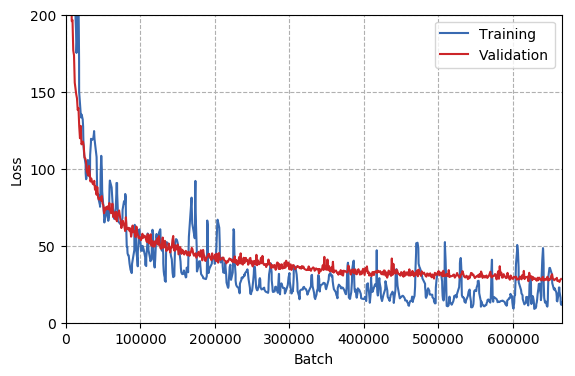
\includegraphics[width=\textwidth]{img/incres_all_loss}
        \vspace*{-.5\baselineskip}
        \caption{Inception-ResNet-v2 loss (108 epochs).\label{fig:best_loss}}
    \end{subfigure}%
    \enspace
    \begin{subfigure}[t]{0.34\textwidth}
    	\centering
        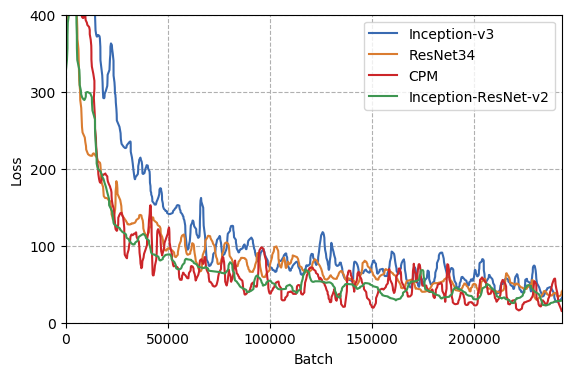
\includegraphics[width=\textwidth]{img/compare_train_loss}
        \vspace*{-.5\baselineskip}
        \caption{Comparison of L\textsubscript{2}-loss at training time.\label{fig:compare_train_loss}}
    \end{subfigure}%
    \enspace
    \begin{subfigure}[t]{0.34\textwidth}
    	\centering
        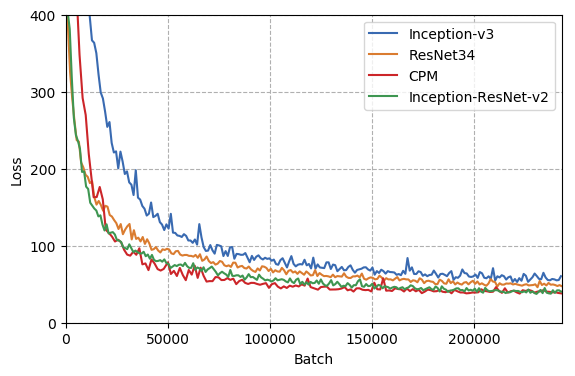
\includegraphics[width=\textwidth]{img/compare_test_loss}
        \vspace*{-.5\baselineskip}
        \caption{Comparison of L\textsubscript{2}-loss at validation time.\label{fig:compare_test_loss}}
    \end{subfigure}%
    \hfill
    \begin{subfigure}[t]{0.34\textwidth}
        \centering
        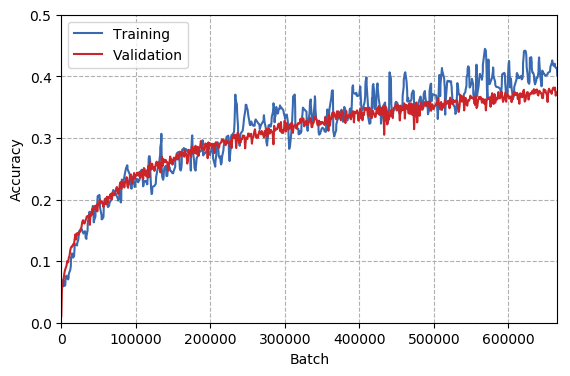
\includegraphics[width=\textwidth]{img/incres_all_acc}
        \vspace*{-.5\baselineskip}
        \caption{Inception-ResNet-v2 accuracy (108 epochs).\label{fig:best_acc}}
    \end{subfigure}%
    \enspace
    \begin{subfigure}[t]{0.34\textwidth}
    	\centering
        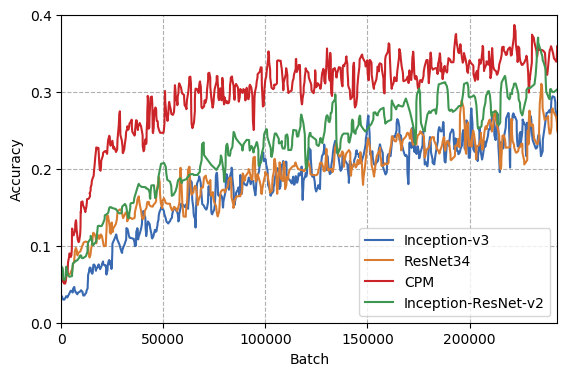
\includegraphics[width=\textwidth]{img/compare_train_acc}
        \vspace*{-.5\baselineskip}
        \caption{Comparison of accuracy at training time.\label{fig:compare_train_acc}}
    \end{subfigure}%
    \enspace
    \begin{subfigure}[t]{0.34\textwidth}
    	\centering
        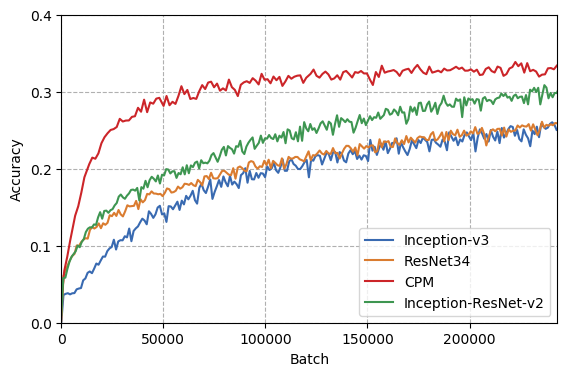
\includegraphics[width=\textwidth]{img/compare_test_acc}
        \vspace*{-.5\baselineskip}
        \caption{Comparison of accuracy at validation time.\label{fig:compare_test_acc}}
    \end{subfigure}
    \vspace*{-.5\baselineskip}
    \caption{Score metrics of Inception-ResNet-v2 and direct comparisons of it with ResNet34, our CPM and Inception-v3.\label{fig:all_graphs}}
    \vspace*{-.5\baselineskip}
\end{figure*} 
 
\section{Discussion}
Considering the comparison of losses for our best model (\autoref{fig:best_loss}) at training and validation time, it is clear that the model started to converge towards the optimal state which may have not been reached even after 108 epochs of training. Another indicator is the increasing prediction accuracy at training and testing time. Significant gains through additional training are not expected without giving the network new data. In comparison to other networks at 45 epochs it gave an accuracy with the largest slope while having the lowest loss. Therefore, it was decided to continue to train it for another 63 epochs.

Sufficiently good results were delivered by our ResNet34 as described earlier. The network's loss was the third smallest and is directly comparable to Inception-ResNet-v2 by using the same approach to loss calculations. The loss was consistently higher while the accuracy was overall lower. This network also trained quicker than Inception-ResNet-v2 but due to different GPUs used, no comparable numbers were produced in time.\\
Comparing different ResNet implementations it is interesting to observe the bottleneck layers which resulted in much worse predictions for the same network as well as advanced techniques presented by \citet{DBLP:journals/corr/HeZR016} detrimentally affecting network performances. The use of Leaky ReLUs is uncertain as of this point, further investigation is required to exclude side-effects of the last layer (\autoref{tab:resnet_summary}) however there was not enough time for this. The last observation which is of interest and lacked time for thorough investigation as well is the shallower implementation of \citet{DBLP:journals/corr/InsafutdinovPAA16} to perform worse than our ResNet34.

Our CPM performed the best for low-epoch runs. Accuracy scores were much higher than any other network while the loss was the lowest. This behaviour is of debate to result in good scores for many epochs as accuracy and loss plateau significantly.  Nevertheless, Kaggle scores evaluated at 20, 30 and 40 epochs (94.89, 97.51, and 86.37) showed increases in performance. Modifications to our CPM (increasing the depth, using larger heatmaps) are expected to increase the fitness.
%One can see that the values of the loss functions (\autoref{fig:best_loss}) have similar values during training and validation at the beginning of the run until approximately 200e+3. However, the model starts to reach the point where more training starts to bring negligible gains at the end of the run as the number of batches increases. Concretely, we start to observe that the training loss continues to decrease, in contrast to the validation loss which plateaus. At that point the increase of number of batches will not introduce the significant gain for the validation loss and the testing (Kaggle) loss.

Inception-v3 exhibited the worst evaluation metrics. The loss decreased less rapidly and finished with overall higher values. A similar accuracy as ResNet34, but higher loss confirmed the received Kaggle score.

Of interesting note was that validation losses did not map with the Kaggle score. The generated validation set and the test images are therefore from different distributions.

The scores received on Kaggle (\autoref{tab:scores_summary}) show minor differences except for ResNet34. Overall, model predictions are robust and exhibit predictable performance for future tasks. 
%ResNet34 performed significantly better than Inception-V3, overall the losses decrease a lot more rapid and the values of the losses are smaller which explains better performance on the testing (Kaggle) set. We trained the model to up to 55 epochs.
%The CPM's implementation generated very low figures in losses and high figures on accuracies during both training and validation compared to other approaches. However, the swift decrease in the losses of CPM is followed by a relatively early plateau compared to the other models. It was therefore decided to not continue to train the CPM implementation for more than 30 epochs. 
%Inception-ResNet-v2 was by far the most performing implementation in terms of the testing (Kaggle) score compared to the other implementations. It significantly outperforms other implementation both in loss and accuracy on the training and validation sets. It was decided to extend the training for more epochs up to 85 epochs.

\section{Conclusion}
In our work we have shown the use of a modified Inception-ResNet-v2 to be a viable alternative to Convolutional Pose Machines in detecting hand joints in images. The performance and fitness of the model show promising results and make it an interesting candidate for future networks on the task of 2D hand pose estimation from single RGB images. With the network being a complex architecture we would like to note its low training throughput in comparison to the other three designs. An interesting approach would be to take the work designed by \citeauthor{DBLP:journals/corr/BulatT16} and have Inception-ResNet-v2 as the part regression network. More involved approaches would include using a model of a hand which is morphed into the prediction of the network and verified to be a reachable pose according to human anatomy. Using this network on videos of hands instead of single RGB images would need further modifications to get smooth predictions with the help of a recurrent network. As of now this network would likely result in high scores for single RGB image poses but sequences of hand-motions are still to be researched. Finally, using our network as the 2D detector of \citet{DBLP:journals/corr/ZimmermannB17} could boost the generated 3D models significantly.

%We proposed a novel solution for the task of hand joint pose estimation from a single RGB image in this paper. The architecture of the proposed model is inspired by the state of the art ResNet designs. The performance of our best performing model was compared to our alternative designs. The image augmentation pipeline is complementing our model to make it able to generalize the data and prevent overfitting. Overall, the system has demonstrated the robustness in performance, although some case as for instance curled hands or multiple people are hard to estimate precisely. The system can be extended for the applications which require the exact joint estimation as for instance sign language recognition from the web camera.
